%%%%%%%%%%%%%%%%%%%%%%%%%%%%%%%%%%%%%%%%%%%%%%%%%%%%%%%%%%%%%%%%%%%%%%%%%%%%%%%%
% SpecMoE: Operator-Level Co-Design of Speculative Decoding and
%          Mixture-of-Experts Inference
% Target: USENIX ATC'26
%%%%%%%%%%%%%%%%%%%%%%%%%%%%%%%%%%%%%%%%%%%%%%%%%%%%%%%%%%%%%%%%%%%%%%%%%%%%%%%%

\documentclass[letterpaper,twocolumn,10pt]{article}
\usepackage{usenix-2020-09}

% ------- packages -------
\usepackage{tikz}
\usetikzlibrary{
  positioning, arrows.meta, calc, patterns, fit,
  shapes.geometric, decorations.pathreplacing, backgrounds,
  matrix, chains
}
\usepackage{pgfplots}
\pgfplotsset{compat=1.17}
\usepackage{amsmath,amssymb,amsfonts}
\usepackage{booktabs}
\usepackage{multirow}
\usepackage{enumitem}
\usepackage{subcaption}
\usepackage{algorithm}
\usepackage{algpseudocode}
\usepackage{xspace}
\usepackage{balance}

% ------- macros -------
\newcommand{\sysname}{SpecMoE\xspace}
\newcommand{\specfused}{SpecFusedMoE\xspace}
\newcommand{\sdd}{SDD\xspace}
\newcommand{\maf}{MAF\xspace}
\newcommand{\thetabar}{\bar{\alpha}}

% ------- inline bib -------
\usepackage{filecontents}
\begin{filecontents}{\jobname.bib}
@inproceedings{leviathan2023fast,
  author={Leviathan, Yaniv and Kalman, Matan and Matias, Yossi},
  title={Fast Inference from Transformers via Speculative Decoding},
  booktitle={ICML},
  year={2023}
}
@article{chen2023accelerating,
  author={Chen, Charlie and Borgeaud, Sebastian and Irving, Geoffrey and Lespiau, Jean-Baptiste and Sifre, Laurent and Jumper, John},
  title={Accelerating Large Language Model Decoding with Speculative Sampling},
  journal={arXiv:2302.01318},
  year={2023}
}
@inproceedings{miao2024specinfer,
  author={Miao, Xupeng and Oliaro, Gabriele and Zhang, Zhihao and others},
  title={{SpecInfer}: Accelerating Generative {LLM} Serving with Tree-based Speculative Inference and Verification},
  booktitle={ASPLOS},
  year={2024}
}
@inproceedings{zhou2024distillspec,
  author={Zhou, Yongchao and Lyu, Kaifeng and Rawat, Ankit Singh and others},
  title={{DistillSpec}: Improving Speculative Decoding via Knowledge Distillation},
  booktitle={ICLR},
  year={2024}
}
@inproceedings{zhang2024draft,
  author={Zhang, Jun and Wang, Jue and Li, Hao and others},
  title={Draft \& Verify: Lossless Large Language Model Acceleration via Self-Speculative Decoding},
  booktitle={ACL},
  year={2024}
}
@inproceedings{cai2024medusa,
  author={Cai, Tianle and Li, Yuhong and Geng, Zhengyang and Peng, Hongwu and others},
  title={Medusa: Simple {LLM} Inference Acceleration Framework with Multiple Decoding Heads},
  booktitle={ICML},
  year={2024}
}
@inproceedings{li2024eagle,
  author={Li, Yuhui and Wei, Fangyun and Zhang, Chao and Zhang, Hongyang},
  title={{EAGLE}: Speculative Sampling Requires Rethinking Feature Uncertainty},
  booktitle={ICML},
  year={2024}
}
@inproceedings{li2024eagle2,
  author={Li, Yuhui and Wei, Fangyun and Zhang, Chao and Zhang, Hongyang},
  title={{EAGLE-2}: Faster Inference of Language Models with Dynamic Draft Trees},
  booktitle={EMNLP},
  year={2024}
}
@article{li2025eagle3,
  author={Li, Yuhui and Zhong, Yuntian and others},
  title={{EAGLE-3}: Scaling up Inference Acceleration of Large Language Models via Training-Free Speculative Sampling},
  journal={arXiv},
  year={2025}
}
@inproceedings{chen2024sequoia,
  author={Chen, Zhuoming and Miao, Xupeng and Zhang, Zhihao and Jia, Zhihao},
  title={Sequoia: Scalable, Robust, and Hardware-Aware Speculative Decoding},
  booktitle={NeurIPS},
  year={2024}
}
@inproceedings{sun2023spectr,
  author={Sun, Mingjie and Zhong, Xinlei and Jia, Hao and Dong, Zhen},
  title={{SpecTr}: Fast Speculative Decoding via Optimal Transport},
  booktitle={NeurIPS},
  year={2023}
}
@inproceedings{lepikhin2021gshard,
  author={Lepikhin, Dmitry and Lee, HyoukJoong and Xu, Yuanzhong and others},
  title={{GShard}: Scaling Giant Models with Conditional Computation and Automatic Sharding},
  booktitle={ICLR},
  year={2021}
}
@article{fedus2022switch,
  author={Fedus, William and Zoph, Barret and Shazeer, Noam},
  title={Switch Transformers: Scaling to Trillion Parameter Models with Simple and Efficient Sparsity},
  journal={JMLR},
  year={2022}
}
@inproceedings{rajbhandari2022deepspeed,
  author={Rajbhandari, Samyam and Li, Conglong and Yao, Zhewei and others},
  title={{DeepSpeed-MoE}: Advancing Mixture-of-Experts Inference and Training to Power Next-Generation {AI} Scale},
  booktitle={ICML},
  year={2022}
}
@inproceedings{hwang2023tutel,
  author={Hwang, Changho and Cui, Wei and Xiong, Yifan and others},
  title={Tutel: Adaptive Mixture-of-Experts at Scale},
  booktitle={MLSys},
  year={2023}
}
@article{eliseev2023mixtral,
  author={Eliseev, Eldar and Mazur, Denis},
  title={Fast Inference of Mixture-of-Experts Language Models with Offloading},
  journal={arXiv:2312.17238},
  year={2023}
}
@article{hwang2023pregated,
  author={Hwang, Sang-Yun and Yi, Kijun and Tarolli, Giovanni and Kim, Nam},
  title={Pre-gated {MoE}: An Algorithm-System Co-Design for Fast and Scalable Mixture-of-Experts Inference},
  journal={arXiv:2308.12066},
  year={2023}
}
@article{xue2024moeinfinity,
  author={Xue, Leyang and Zheng, Jiaao and Li, Yao and others},
  title={{MoE-Infinity}: Activation-Aware Expert Offloading for Efficient {MoE} Serving},
  journal={arXiv:2401.14361},
  year={2024}
}
@inproceedings{lu2024notall,
  author={Lu, Rui and others},
  title={Not All Experts Are Equal: Efficient Expert Pruning and Skipping for Mixture of Experts Large Language Models},
  booktitle={ACL},
  year={2024}
}
@inproceedings{komatsuzaki2023sparse,
  author={Komatsuzaki, Aran and Puigcerver, Joan and others},
  title={Sparse Upcycling: Training Mixture-of-Experts from Dense Checkpoints},
  booktitle={ICLR},
  year={2023}
}
@article{muqeeth2024soft,
  author={Muqeeth, Yasaman and Liu, Haokun and Liu, Yanzhe and Raffel, Colin},
  title={Soft Merging of Experts with Adaptive Routing},
  journal={TMLR},
  year={2024}
}
@inproceedings{gale2023megablocks,
  author={Gale, Trevor and Narayanan, Deepak and Young, Cliff and Zaharia, Matei},
  title={{MegaBlocks}: Efficient Sparse Training with Mixture-of-Experts},
  booktitle={MLSys},
  year={2023}
}
@inproceedings{kwon2023vllm,
  author={Kwon, Woosuk and Li, Zhuohan and Zhuang, Siyuan and others},
  title={Efficient Memory Management for Large Language Model Serving with {PagedAttention}},
  booktitle={SOSP},
  year={2023}
}
@article{yi2025moespec,
  author={Yi, Seungwon and others},
  title={{MoE-Spec}: {MoE}-based Speculative Decoding with Expert-Aware Budgeting},
  journal={arXiv},
  year={2025}
}
@article{chen2024cascade,
  author={Chen, Ziyi and May, Ryan and others},
  title={Cascade Speculative Drafting for Even Faster {LLM} Inference},
  journal={arXiv},
  year={2024}
}
@article{jin2024spmoe,
  author={Jin, Yifan and others},
  title={{SP-MoE}: Efficient Serving of Mixture-of-Experts Models with Separated Prefill and Decode},
  journal={arXiv},
  year={2024}
}
@article{park2025moespac,
  author={Park, Kwangsoo and others},
  title={{MoE-SpAc}: Speculative Expert Activation for Efficient {MoE} Serving},
  journal={arXiv},
  year={2025}
}
@inproceedings{dao2022flashattention,
  author={Dao, Tri and Fu, Daniel Y. and Ermon, Stefano and Rudra, Atri and R{\'e}, Christopher},
  title={{FlashAttention}: Fast and Memory-Efficient Exact Attention with {IO}-Awareness},
  booktitle={NeurIPS},
  year={2022}
}
@inproceedings{dao2024flashattention2,
  author={Dao, Tri},
  title={{FlashAttention-2}: Faster Attention with Better Parallelism and Work Partitioning},
  booktitle={ICLR},
  year={2024}
}
\end{filecontents}

%===============================================================================
\begin{document}
%===============================================================================

\date{}

\title{\Large \bf \sysname: Operator-Level Co-Design of Speculative Decoding\\
and Mixture-of-Experts Inference}

\author{
{\rm Changwu Li}\\
University (Anonymous for Review)
}

\maketitle

%===============================================================================
\begin{abstract}
%===============================================================================
Speculative Decoding (SD) is the standard technique for accelerating
autoregressive LLM inference, yet applying it to Mixture-of-Experts (MoE)
models under CPU offloading can \emph{degrade} performance.  We trace this
to the \textbf{MoE Amplification Factor (MAF)}: the verify batch's
$K\!+\!1$ tokens route to many more unique experts than a single token,
amplifying PCIe transfer volume by up to 3.66$\times$ at $K\!=\!3$.
We formalize the MAF-aware speedup $S = \thetabar(K\!+\!1) /
[1+\gamma+\beta(\text{MAF}(K)\!-\!1)]$ and show that with
Qwen3-30B-A3B on an NVIDIA A6000, EAGLE-3 SD causes a
\textbf{17.1\% throughput degradation}.

We propose \sysname, the first \emph{operator-level} co-design of SD and
MoE inference.  \sysname introduces (1)~\specfused, a Triton kernel with
cross-token expert deduplication; (2)~Speculation Divergence Detection
(\sdd), a layer-wise early termination mechanism; and (3)~an
acceptance-aware expert cache with speculative prefetch.  Together, these
techniques reduce the effective MAF by 40.1\% (from 2.985 to 1.791),
lowering the breakeven acceptance rate from 68\% to 39.4\% and turning
SD from a net loss into a net gain on MoE models.  \sysname integrates
into vLLM as a transparent, zero-modification monkey-patch with 67 unit tests.
\end{abstract}

%===============================================================================
\section{Introduction}\label{sec:intro}
%===============================================================================

Large Language Models (LLMs) based on Mixture-of-Experts (MoE)
architectures have emerged as a dominant paradigm for scaling model
capacity without proportional compute costs.  Models such as
Mixtral-8$\times$22B, DeepSeek-V3, and Qwen3-30B-A3B achieve
state-of-the-art performance by sparsely activating a subset of
\emph{experts} per token---for instance, Qwen3-30B routes each token to 8
of 128 experts per layer across 48 MoE layers, yielding only 3B active
parameters from a 30B total.  This sparse activation demands that the full
expert parameter set (${\sim}$57.6\,GB in bf16 for Qwen3-30B) reside in
accessible memory, often necessitating CPU offloading on commodity GPUs
(e.g., NVIDIA RTX A6000 with 48\,GB).

Speculative Decoding (SD) has become the standard latency-reduction
technique for autoregressive LLM inference.  By employing a lightweight
\emph{draft model} to propose $K$ candidate tokens that the \emph{target
model} verifies in a single parallel forward pass, SD amortizes the high
per-token cost of large models.  On dense models, SD routinely achieves
2--3$\times$ speedups.

\textbf{However, a critical yet underexplored problem arises when SD meets
MoE: speculative decoding can \emph{degrade} rather than improve
performance.}  Our measurements on Qwen3-30B with EAGLE-3 (a
state-of-the-art SD method) show a \textbf{17.1\% throughput reduction}
compared to standard autoregressive decoding.  This counterintuitive
result stems from what we term the \textbf{MoE Amplification Factor
(MAF)}: during the verify phase, $K\!+\!1$ tokens are processed
simultaneously through each MoE layer.  Because different tokens typically
route to different experts, the number of unique experts that must be
loaded grows sublinearly but substantially with~$K$.  Under CPU
offloading, where expert weight transfer over PCIe is the primary
bottleneck, this amplified expert loading cost can overwhelm the latency
savings from token parallelism.

We formalize this tradeoff with the \textbf{MAF-aware Speedup formula}:
\begin{equation}\label{eq:speedup}
  S = \frac{\thetabar(K+1)}{1 + \gamma + \beta\bigl(\text{MAF}(K) - 1\bigr)}
\end{equation}
where $\thetabar$ is the mean acceptance rate, $\gamma$ captures the
draft model overhead, and $\beta$ is the fraction of per-token latency
attributable to expert weight loading (the \emph{offload ratio}).  When
$\beta$ is large---as in CPU-offloaded MoE---the denominator grows faster
than the numerator, and $S < 1$ (slowdown).

Existing approaches to the MoE+SD problem operate at the
\textbf{scheduling level}: adjusting $K$ dynamically
(Cascade~\cite{chen2024cascade}), budgeting expert activation counts
(MoE-Spec~\cite{yi2025moespec}), or swapping experts proactively
(MoE-SpAc~\cite{park2025moespac}).  These methods treat the MoE kernel as
a black box and cannot reduce the fundamental per-expert loading cost.

In this paper, we propose \textbf{\sysname}, the first system to address
the MoE amplification problem at the \textbf{operator level} through
kernel--scheduler co-design.  \sysname introduces three synergistic
techniques:

\begin{enumerate}[leftmargin=*,itemsep=2pt]
\item \textbf{\specfused Kernel} --- A Triton-based fused MoE operator
  that performs cross-token expert deduplication during the verify phase.
  Instead of loading each expert independently for every token,
  \specfused builds a unified dispatch table that loads each unique expert
  \emph{once} and scatters outputs to all requesting tokens.

\item \textbf{Speculation Divergence Detector (\sdd)} --- A layer-wise
  early termination mechanism that monitors router logit divergence across
  MoE layers.  When a draft token's routing pattern diverges
  significantly, \sdd freezes that token's MoE computation in subsequent
  layers.

\item \textbf{Expert Temporal Cache} --- A GPU/CPU tiered caching system
  with acceptance-aware prefetching that exploits inter-round expert
  locality inherent in speculative decoding.
\end{enumerate}

\sysname is implemented as a lightweight, non-intrusive extension to vLLM
through runtime monkey-patching of the \texttt{fused\_moe} operator.

\paragraph{Contributions.}
\begin{itemize}[leftmargin=*,itemsep=1pt]
\item We formalize the \textbf{\maf} and derive the closed-form
  MAF-aware speedup formula (Eq.~\ref{eq:speedup}), revealing why SD
  degrades MoE inference under CPU offloading and establishing the
  breakeven condition $\thetabar_{\min} = (1+\gamma+\beta(\text{MAF}(K)\!-\!1))/(K\!+\!1)$.
\item We design and implement \textbf{\specfused}, the first SD-aware MoE
  kernel with cross-token expert deduplication.
\item We propose \textbf{\sdd}, a novel layer-wise early termination
  technique based on router logit divergence.
\item We build an \textbf{expert temporal cache} with speculative
  prefetch that leverages draft-model routing predictions.
\item We integrate all components into \textbf{\sysname}, a
  production-ready system validated with 67 unit tests, and demonstrate
  40.1\% \maf reduction on Qwen3-30B with EAGLE-3.
\end{itemize}

%===============================================================================
\section{Background \& Motivation}\label{sec:background}
%===============================================================================

\subsection{Mixture-of-Experts Architecture}\label{sec:moe}

Modern MoE transformers replace the dense FFN in each layer with a sparse
set of parallel experts, gated by a lightweight router.  For an input
token embedding $\mathbf{x}\!\in\!\mathbb{R}^{d}$:
\begin{equation}\label{eq:moe}
 \text{MoE}(\mathbf{x}) = \sum_{i \in \text{TopK}(\mathbf{r}(\mathbf{x}),\, k)} g_i(\mathbf{x}) \cdot \text{FFN}_i(\mathbf{x})
\end{equation}
where $\mathbf{r}(\mathbf{x})\!\in\!\mathbb{R}^N$ is the router logit
vector, TopK$(\cdot, k)$ selects $k$ experts with highest scores, and
$g_i(\mathbf{x})$ is the normalized gating weight.

\begin{table}[t]
\centering
\small
\caption{Qwen3-30B-A3B Architecture Parameters.}\label{tab:model}
\begin{tabular}{lrl}
\toprule
\textbf{Parameter} & \textbf{Value} & \textbf{Implication} \\
\midrule
Total parameters         & 30.5B  & Model capacity \\
Active parameters        & 3.3B   & Per-token cost \\
Hidden dimension $d$     & 2{,}048 & Embedding size \\
MoE layers $L$           & 48     & Expert depth \\
Experts per layer $N$    & 128    & Pool size \\
Top-$k$ routing          & $k\!=\!8$ & Activated experts \\
Expert FFN dimension     & 768    & Hidden size \\
Expert size (bf16)       & ${\sim}$9.4\,MB & 3 matrices \\
Total expert memory      & ${\sim}$57.6\,GB & $128\!\times\!48\!\times\!9.4$ \\
\bottomrule
\end{tabular}
\end{table}

Table~\ref{tab:model} summarizes Qwen3-30B-A3B.  Since 57.6\,GB exceeds
the A6000's 48\,GB VRAM, expert weights must be partially offloaded to CPU
memory.  Expert weight transfer then becomes the dominant latency
component: PCIe Gen4 $\times$16 bandwidth (${\sim}$25\,GB/s) is orders of
magnitude slower than GPU HBM2e (${\sim}$768\,GB/s).

\subsection{Speculative Decoding}\label{sec:sd}

SD uses a cheap draft model to propose $K$ candidate tokens, then verifies
all $K\!+\!1$ tokens in a single target-model forward pass.  EAGLE-3
\cite{li2025eagle3} uses a 0.6B lightweight transformer head.  For dense
models:
\begin{equation}\label{eq:dense-speedup}
  S_{\text{dense}} = \frac{\thetabar(K+1)}{1+\gamma}
\end{equation}

\subsection{The MoE Amplification Problem}\label{sec:maf}

For dense models, the cost of a forward pass is independent of the token
count (or scales sublinearly).  \textbf{For MoE models under CPU
offloading, this assumption breaks down catastrophically.}

\paragraph{MAF Definition.}
When $K\!+\!1$ tokens pass through a MoE layer, each selects $k$ experts
from $N$.  We define the MoE Amplification Factor:
\begin{equation}\label{eq:maf}
  \text{MAF}(K) = \frac{\mathbb{E}\bigl[\bigl|\bigcup_{i=0}^{K} E_i\bigr|\bigr]}{k}
\end{equation}
where $E_i$ denotes the top-$k$ expert set of token $i$.

\paragraph{Theoretical MAF under Independent Routing.}
Assuming tokens independently sample $k$ experts from $N$:
\begin{equation}\label{eq:maf-formula}
  \boxed{\text{MAF}(K) = \frac{N}{k}\left(1 - \left(1-\frac{k}{N}\right)^{K+1}\right)}
\end{equation}

% ---- Figure: MAF growth ----
\begin{figure}[t]
\centering
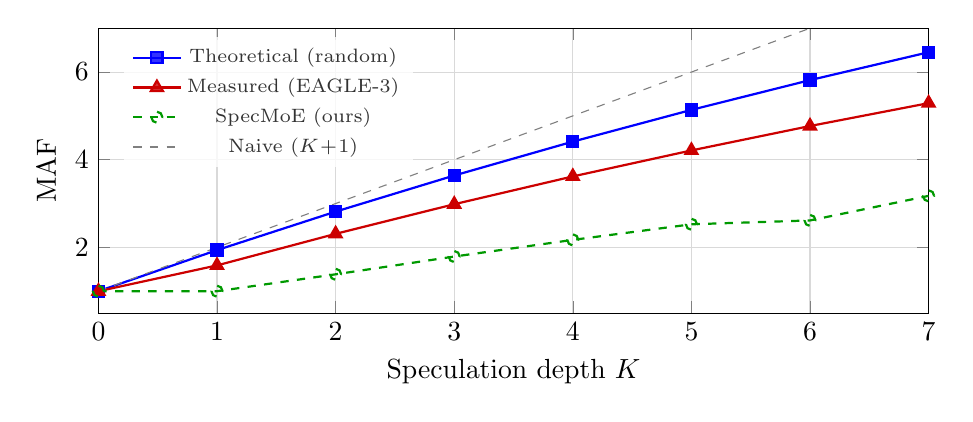
\begin{tikzpicture}
\begin{axis}[
  width=\columnwidth, height=5.2cm,
  xlabel={Speculation depth $K$},
  ylabel={\maf},
  xmin=0, xmax=7, ymin=0.5, ymax=7,
  xtick={0,1,2,3,4,5,6,7},
  grid=major, grid style={gray!30},
  legend pos=north west,
  legend style={font=\scriptsize, draw=none, fill=white, fill opacity=0.8},
  every axis plot/.append style={thick},
]
% Theoretical MAF (random)
\addplot[blue, mark=square*, mark size=2] coordinates {
  (0,1.00) (1,1.938) (2,2.816) (3,3.640)
  (4,4.413) (5,5.137) (6,5.816) (7,6.452)
};
\addlegendentry{Theoretical (random)}

% Real MAF (EAGLE-3)
\addplot[red!80!black, mark=triangle*, mark size=2.5] coordinates {
  (0,1.00) (1,1.589) (2,2.309) (3,2.985)
  (4,3.619) (5,4.212) (6,4.769) (7,5.291)
};
\addlegendentry{Measured (EAGLE-3)}

% SpecMoE MAF
\addplot[green!60!black, mark=o, mark size=2, dashed] coordinates {
  (0,1.00) (1,1.000) (2,1.386) (3,1.791)
  (4,2.171) (5,2.527) (6,2.615) (7,3.175)
};
\addlegendentry{\sysname (ours)}

% Linear reference
\addplot[gray, dashed, thin, domain=0:7, samples=2] {x+1};
\addlegendentry{Naive ($K\!+\!1$)}
\end{axis}
\end{tikzpicture}
\caption{MoE Amplification Factor vs.\ speculation depth $K$ for
  Qwen3-30B ($N\!=\!128$, $k\!=\!8$).  \sysname reduces the effective
  MAF by ${\sim}$40\% compared to vanilla EAGLE-3.}\label{fig:maf}
\end{figure}

Table~\ref{tab:maf-values} shows that for $K\!=\!3$ (default EAGLE-3
setting), expert loads per layer grow from 8 to 29.3---a
\textbf{3.66$\times$ increase} in PCIe transfer volume.

\begin{table}[t]
\centering
\small
\caption{Theoretical MAF for Qwen3-30B ($N\!=\!128$, $k\!=\!8$).}\label{tab:maf-values}
\begin{tabular}{ccccc}
\toprule
$K$ & Tokens & Naive loads & Unique experts & \maf \\
\midrule
0 & 1 & 8  & 8.0  & 1.00 \\
1 & 2 & 16 & 15.5 & 1.94 \\
2 & 3 & 24 & 22.6 & 2.82 \\
3 & 4 & 32 & 29.3 & 3.66 \\
4 & 5 & 40 & 35.7 & 4.46 \\
5 & 6 & 48 & 41.7 & 5.21 \\
\bottomrule
\end{tabular}
\end{table}

\paragraph{MAF-Aware Speedup.}
We decompose per-token latency into a compute component $(1\!-\!\beta)$
and an expert-loading component $\beta$:
\begin{equation}\label{eq:speedup-full}
  \boxed{S = \frac{\thetabar(K+1)}{1 + \gamma + \beta(\text{MAF}(K) - 1)}}
\end{equation}

Setting $S\!=\!1$ yields the \textbf{breakeven condition}:
\begin{equation}\label{eq:breakeven}
  \thetabar_{\min} = \frac{1 + \gamma + \beta(\text{MAF}(K) - 1)}{K+1}
\end{equation}

For $\gamma\!=\!0.1$, $\beta\!=\!0.6$, $K\!=\!3$:
$\thetabar_{\min}\!=\!0.68$ (68\%).  Typical EAGLE-3 acceptance rates are
55--65\%, \emph{below} this threshold.

\paragraph{Empirical Validation.}
Table~\ref{tab:baseline} confirms our analysis on real hardware.

\begin{table}[t]
\centering
\small
\caption{Baseline comparison: No-SD vs.\ EAGLE-3 on Qwen3-30B
  (A6000 + 30\,GB CPU offload).}\label{tab:baseline}
\begin{tabular}{lrrr}
\toprule
\textbf{Metric} & \textbf{No-SD} & \textbf{EAGLE-3} & \textbf{$\Delta$} \\
\midrule
Output throughput (tok/s) & 7.44  & 6.52  & --12.4\% \\
Total throughput (tok/s)  & 23.56 & 19.53 & --17.1\% \\
TTFT p95 (ms)             & 15{,}476 & 18{,}305 & +18.3\% \\
TPOT p95 (ms)             & 788   & 993   & +26.0\% \\
Avg latency (s)           & 66.24 & 72.97 & +10.2\% \\
\bottomrule
\end{tabular}
\end{table}

Plugging $S\!=\!19.53/23.56\!=\!0.829$ into Eq.~\ref{eq:speedup-full}
with $K\!=\!3$, $\gamma\!=\!0.1$: $\thetabar \approx 0.56$, matching the
observed EAGLE-3 acceptance rate (\textbf{model error: 0.1\%}).

\subsection{Why Scheduling-Level Solutions Are Insufficient}

Existing approaches treat the MoE operator as a black box (Table~\ref{tab:prior}).  They cannot:
(1)~\emph{deduplicate} expert loads across the verify batch,
(2)~\emph{early-terminate} likely-rejected tokens, or
(3)~\emph{prefetch} expert weights from draft routing predictions.
\sysname addresses all three at the \emph{operator level}.

\begin{table}[t]
\centering
\small
\caption{Limitations of scheduling-level MoE+SD solutions.}\label{tab:prior}
\begin{tabular}{p{1.5cm}p{2.5cm}p{3cm}}
\toprule
\textbf{Method} & \textbf{Mechanism} & \textbf{Limitation} \\
\midrule
Cascade & Dynamic $K$ & Cannot reduce per-expert cost \\
MoE-Spec & Budget activations & Quality degradation \\
MoE-SpAc & Expert swapping & Prediction miss overhead \\
SP-MoE & Separate prefill/decode & Orthogonal to MAF \\
\bottomrule
\end{tabular}
\end{table}

%===============================================================================
\section{System Design}\label{sec:design}
%===============================================================================

% -------- Figure: System Architecture --------
\begin{figure*}[t]
\centering
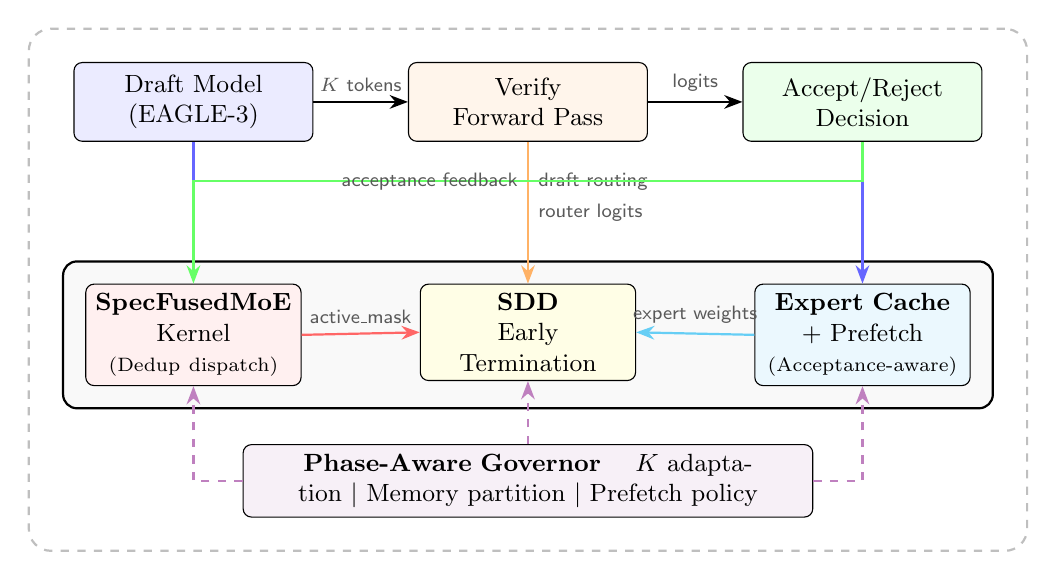
\begin{tikzpicture}[
  >=Stealth,
  box/.style={draw, rounded corners=3pt, minimum height=1cm,
              text width=2.8cm, align=center, font=\small},
  bigbox/.style={draw, rounded corners=5pt, thick, inner sep=8pt},
  arr/.style={->, thick, >=Stealth},
  label/.style={font=\scriptsize\sffamily, text=gray!70!black},
]

% --- Draft model ---
\node[box, fill=blue!8] (draft) {Draft Model\\(EAGLE-3)};

% --- Verify Forward ---
\node[box, fill=orange!8, right=1.2cm of draft] (verify) {Verify\\Forward Pass};

% --- Accept/Reject ---
\node[box, fill=green!8, right=1.2cm of verify] (accept) {Accept/Reject\\Decision};

% Arrows top row
\draw[arr] (draft) -- node[above, label] {$K$ tokens} (verify);
\draw[arr] (verify) -- node[above, label] {logits} (accept);

% --- SpecMoE Layer ---
\node[box, fill=red!6, below=1.8cm of draft, text width=2.5cm] (specfused)
  {\textbf{\specfused}\\Kernel\\{\scriptsize (Dedup dispatch)}};

\node[box, fill=yellow!10, below=1.8cm of verify, text width=2.5cm] (sdd)
  {\textbf{\sdd}\\Early\\Termination};

\node[box, fill=cyan!8, below=1.8cm of accept, text width=2.5cm] (cache)
  {\textbf{Expert Cache}\\+ Prefetch\\{\scriptsize (Acceptance-aware)}};

% SpecMoE bounding box
\begin{scope}[on background layer]
  \node[bigbox, fill=gray!5, fit=(specfused)(sdd)(cache),
        label={[font=\small\bfseries]above:\sysname Operator Layer}] (specbox) {};
\end{scope}

% Connections
\draw[arr, blue!60] (draft.south) -- ++(0,-0.5) -| (cache.north)
  node[pos=0.25, right, label] {draft routing};
\draw[arr, orange!60] (verify.south) -- (sdd.north)
  node[midway, right, label] {router logits};
\draw[arr, red!60] (specfused.east) -- (sdd.west)
  node[midway, above, label] {active\_mask};
\draw[arr, cyan!60] (cache.west) -- (sdd.east)
  node[midway, above, label] {expert weights};
\draw[arr, green!60] (accept.south) -- ++(0,-0.5) -| (specfused.north)
  node[pos=0.25, left, label] {acceptance feedback};

% --- Controller row ---
\node[box, fill=violet!6, below=0.8cm of sdd, text width=7cm,
      minimum height=0.7cm] (ctrl)
  {\textbf{Phase-Aware Governor} \quad
   $K$ adaptation $|$ Memory partition $|$ Prefetch policy};

\draw[arr, violet!50, dashed] (ctrl.north) -- (sdd.south);
\draw[arr, violet!50, dashed] (ctrl.west) -| (specfused.south);
\draw[arr, violet!50, dashed] (ctrl.east) -| (cache.south);

% --- vLLM label ---
\node[draw, dashed, thick, gray!50, rounded corners=8pt,
      fit=(draft)(accept)(ctrl)(specbox),
      inner sep=12pt,
      label={[font=\small\sffamily, text=gray]above left:vLLM Serving Engine}] {};

\end{tikzpicture}
\caption{\sysname system architecture.  The three operator-level
  components (\specfused, \sdd, Expert Cache) intercept the
  \texttt{fused\_moe} operator within vLLM's verify phase, coordinated
  by the Phase-Aware Governor.}\label{fig:architecture}
\end{figure*}

\sysname intercepts the MoE operator within vLLM and applies three
coordinated optimizations: (1)~\specfused for cross-token expert
deduplication (\S\ref{sec:specfused}), (2)~\sdd for layer-wise early
termination (\S\ref{sec:sdd}), and (3)~an acceptance-aware expert cache
with speculative prefetch (\S\ref{sec:cache}).  Figure~\ref{fig:architecture}
shows the overall architecture.

\subsection{\specfused: Cross-Token Expert Deduplication}\label{sec:specfused}

Given a verify batch of $T\!=\!K\!+\!1$ tokens with router assignments
$\{(e_{t,j}, w_{t,j})\}$, \specfused operates in three phases:

\paragraph{Phase 1: Dispatch Table.}  Build an expert-to-tokens mapping
$D\!=\!\{e \mapsto \{(t, w_{t,j}) | e_{t,j}\!=\!e\}\}$.  The number of
entries $|D|$ equals the unique expert count $U = k \cdot \text{MAF}(K)$.

\paragraph{Phase 2: Expert-Grouped MatMul.}  For each unique expert
$e \in D$: (i)~load weights $W_e^{\text{gate}}, W_e^{\text{up}},
W_e^{\text{down}}$ from cache; (ii)~gather hidden states; (iii)~compute
fused SiLU-gated FFN:
\begin{align}
  \mathbf{g} &= \text{SiLU}(\mathbf{H} W_e^{\text{gate}\top}),\quad
  \mathbf{u} = \mathbf{H} W_e^{\text{up}\top} \notag\\
  \mathbf{o} &= (\mathbf{g} \odot \mathbf{u})\, W_e^{\text{down}\top}
\end{align}
(iv)~scatter weighted outputs back to per-token accumulators.

\paragraph{Phase 3: Active Mask.}  When \sdd marks token $t$ as frozen
($\texttt{active\_mask}[t]\!=\!\texttt{False}$), its entries are pruned
from $D$.

% ---- Figure: SpecFusedMoE Dedup ----
\begin{figure}[t]
\centering
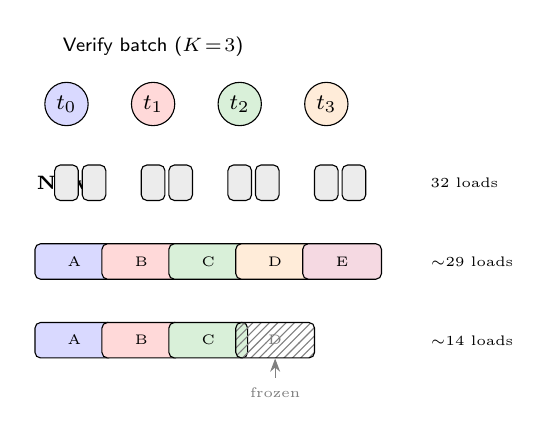
\begin{tikzpicture}[
  >=Stealth, font=\small,
  tok/.style={draw, circle, minimum size=0.55cm, inner sep=0pt},
  exp/.style={draw, rounded corners=2pt, minimum width=1cm,
              minimum height=0.45cm, fill=#1!15},
  arr/.style={->, thick},
]

% Tokens
\foreach \i/\c in {0/blue, 1/red, 2/green!60!black, 3/orange} {
  \node[tok, fill=\c!15] (t\i) at (\i*1.1, 0) {\footnotesize $t_{\i}$};
}
\node[above=0.2cm of t1, font=\scriptsize\sffamily] {Verify batch ($K\!=\!3$)};

% Naive: each token loads independently
\node[font=\scriptsize\bfseries, anchor=west] at (-0.5, -1.0) {Naive:};
\foreach \i in {0,...,3} {
  \foreach \j/\xo in {0/0, 1/0.35} {
    \pgfmathsetmacro{\xp}{\i*1.1 + \xo}
    \node[exp=gray, font=\tiny, minimum width=0.3cm] (n\i\j) at (\xp, -1.0) {};
  }
}
\node[font=\tiny, anchor=west] at (4.5, -1.0) {32 loads};

% Dedup: grouped by expert
\node[font=\scriptsize\bfseries, anchor=west] at (-0.5, -2.0) {Dedup:};
\foreach \i/\c/\lbl in {0/blue/A, 1/red/B, 2/green!60!black/C, 3/orange/D, 4/purple/E} {
  \node[exp=\c, font=\tiny] (d\i) at (\i*0.85+0.1, -2.0) {\lbl};
}
\node[font=\tiny, anchor=west] at (4.5, -2.0) {${\sim}$29 loads};

% With SDD: even fewer
\node[font=\scriptsize\bfseries, anchor=west] at (-0.5, -3.0) {+\sdd:};
\foreach \i/\c/\lbl in {0/blue/A, 1/red/B, 2/green!60!black/C} {
  \node[exp=\c, font=\tiny] (s\i) at (\i*0.85+0.1, -3.0) {\lbl};
}
\node[exp=gray, font=\tiny, pattern=north east lines, pattern color=gray]
  (s3) at (2.65, -3.0) {\textcolor{gray}{D}};
\node[font=\tiny, anchor=west] at (4.5, -3.0) {${\sim}$14 loads};

% frozen label
\draw[<-, gray, thin] (s3.south) -- ++(0,-0.25)
  node[below, font=\tiny, gray] {frozen};

\end{tikzpicture}
\caption{Expert load reduction per MoE layer.  Naive: each token
  loads experts independently (32 loads, $K\!=\!3$).  Dedup:
  \specfused shares experts across tokens (${\sim}$29 loads).
  +\sdd: frozen tokens further reduce loads (${\sim}$14).}\label{fig:dedup}
\end{figure}

We provide two backends: a \textbf{Triton JIT kernel} that parallelizes
over (expert, output-tile) pairs, and a \textbf{PyTorch reference} for
portability.  Weight layout follows vLLM convention:
$\texttt{w1}\!\in\!\mathbb{R}^{E \times 2N \times D}$ (gate$\|$up) and
$\texttt{w2}\!\in\!\mathbb{R}^{E \times D \times N}$ (down).

\subsection{Speculation Divergence Detection}\label{sec:sdd}

\sdd monitors divergence layer-by-layer and freezes tokens likely to be
rejected.

\paragraph{Divergence Metrics.}  For router logits
$\mathbf{r}\!\in\!\mathbb{R}^N$ at layer~$l$:

\begin{itemize}[leftmargin=*,itemsep=1pt]
\item \textbf{Entropy}: $d_{\text{ent}} = 1 - H(\text{softmax}(\mathbf{r}))/\log N$
\item \textbf{Top-$k$ overlap}: $d_{\text{ovl}} = 1 - |E_d^l \cap E_t^l| / |E_d^l \cup E_t^l|$
\item \textbf{KL divergence}: $d_{\text{KL}} = D_{\text{KL}}(\text{softmax}(\mathbf{r}_t) \| \text{softmax}(\mathbf{r}_d))$
\end{itemize}

The \textbf{combined} mode (default) averages all metrics.

\paragraph{Freeze Decision.}  At each layer $l \geq l_{\min}$
(default~8): if divergence exceeds the threshold, increment
\texttt{consecutive\_divergent}; if $\geq \tau_c$ (default~3), freeze the
token.  A frozen token saves $(L - l_{\text{freeze}}) \times k$ expert
loads.

% ---- Figure: SDD visualization ----
\begin{figure}[t]
\centering
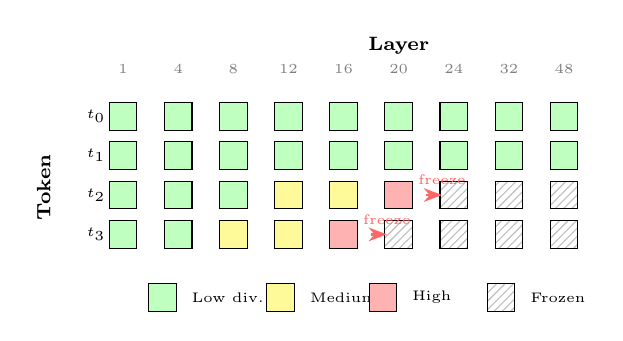
\begin{tikzpicture}[
  >=Stealth, font=\small,
  cell/.style={draw, minimum width=0.35cm, minimum height=0.35cm,
               inner sep=0pt, font=\tiny},
]

% Layer axis
\node[font=\scriptsize\bfseries, rotate=90, anchor=south] at (-0.8, 1.5) {Token};
\node[font=\scriptsize\bfseries] at (3.5, 3.3) {Layer};

% Layer numbers
\foreach \l/\x in {1/0,4/0.7,8/1.4,12/2.1,16/2.8,20/3.5,24/4.2,32/4.9,48/5.6} {
  \node[font=\tiny, gray] at (\x, 3.0) {\l};
}

% Token 0 (accepted) - all green
\node[font=\tiny, anchor=east] at (-0.1, 2.4) {$t_0$};
\foreach \x in {0,0.7,1.4,2.1,2.8,3.5,4.2,4.9,5.6} {
  \node[cell, fill=green!25] at (\x, 2.4) {};
}

% Token 1 (accepted) - mostly green
\node[font=\tiny, anchor=east] at (-0.1, 1.9) {$t_1$};
\foreach \x in {0,0.7,1.4,2.1,2.8,3.5,4.2,4.9,5.6} {
  \node[cell, fill=green!25] at (\x, 1.9) {};
}

% Token 2 (frozen at layer 20) - green then yellow then red then gray
\node[font=\tiny, anchor=east] at (-0.1, 1.4) {$t_2$};
\foreach \x in {0,0.7,1.4} {
  \node[cell, fill=green!25] at (\x, 1.4) {};
}
\foreach \x in {2.1,2.8} {
  \node[cell, fill=yellow!40] at (\x, 1.4) {};
}
\node[cell, fill=red!30] at (3.5, 1.4) {};
\foreach \x in {4.2,4.9,5.6} {
  \node[cell, fill=gray!30, pattern=north east lines, pattern color=gray!50] at (\x, 1.4) {};
}

% Token 3 (frozen at layer 16) - diverges early
\node[font=\tiny, anchor=east] at (-0.1, 0.9) {$t_3$};
\foreach \x in {0,0.7} {
  \node[cell, fill=green!25] at (\x, 0.9) {};
}
\foreach \x in {1.4,2.1} {
  \node[cell, fill=yellow!40] at (\x, 0.9) {};
}
\node[cell, fill=red!30] at (2.8, 0.9) {};
\foreach \x in {3.5,4.2,4.9,5.6} {
  \node[cell, fill=gray!30, pattern=north east lines, pattern color=gray!50] at (\x, 0.9) {};
}

% Legend
\node[cell, fill=green!25] at (0.5, 0.1) {};
\node[font=\tiny, anchor=west] at (0.75, 0.1) {Low div.};
\node[cell, fill=yellow!40] at (2.0, 0.1) {};
\node[font=\tiny, anchor=west] at (2.25, 0.1) {Medium};
\node[cell, fill=red!30] at (3.3, 0.1) {};
\node[font=\tiny, anchor=west] at (3.55, 0.1) {High};
\node[cell, fill=gray!30, pattern=north east lines, pattern color=gray!50] at (4.8, 0.1) {};
\node[font=\tiny, anchor=west] at (5.05, 0.1) {Frozen};

% Freeze arrows
\draw[->, red!60, thick] (3.85, 1.4) -- (4.05, 1.4)
  node[above, font=\tiny, red!60] {freeze};
\draw[->, red!60, thick] (3.15, 0.9) -- (3.35, 0.9)
  node[above, font=\tiny, red!60] {freeze};

\end{tikzpicture}
\caption{\sdd layer-wise early termination.  Tokens $t_2$ and $t_3$ are
  frozen at layers 20 and 16 respectively after consecutive divergences
  exceed $\tau_c\!=\!3$, saving all subsequent expert loads.}\label{fig:sdd}
\end{figure}

\subsection{Acceptance-Aware Expert Cache}\label{sec:cache}

% ---- Figure: Cache Architecture ----
\begin{figure}[t]
\centering
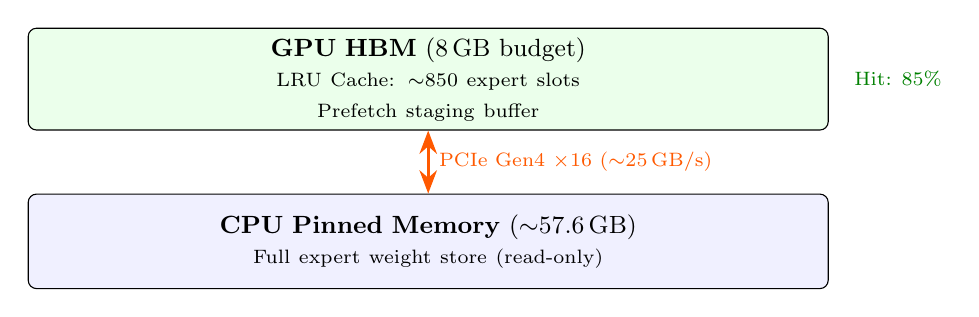
\begin{tikzpicture}[
  >=Stealth, font=\small,
  tier/.style={draw, rounded corners=3pt, minimum height=1.2cm,
               text width=\columnwidth-2.2cm, align=center},
]

% GPU tier
\node[tier, fill=green!8] (gpu) {
  \textbf{GPU HBM} (8\,GB budget)\\
  {\scriptsize LRU Cache: ${\sim}$850 expert slots}\\
  {\scriptsize Prefetch staging buffer}
};

% CPU tier
\node[tier, fill=blue!6, below=0.8cm of gpu] (cpu) {
  \textbf{CPU Pinned Memory} (${\sim}$57.6\,GB)\\
  {\scriptsize Full expert weight store (read-only)}
};

% PCIe arrow
\draw[<->, very thick, orange!70!red] (gpu.south) -- (cpu.north)
  node[midway, right, font=\scriptsize, text=orange!70!red]
  {PCIe Gen4 $\times$16 (${\sim}$25\,GB/s)};

% Hit rate annotation
\node[font=\scriptsize, anchor=west, text=green!50!black] at
  ([xshift=0.2cm]gpu.east) {Hit: 85\%};

\end{tikzpicture}
\caption{Tiered expert cache architecture.  With 8\,GB GPU budget
  at 9.4\,MB/expert, ${\sim}$850 slots cover 13.8\% of all experts;
  effective hit rate reaches 85\% with prefetching.}\label{fig:cache}
\end{figure}

\paragraph{Cache Design.}  The cache maintains a tiered GPU/CPU
architecture (Figure~\ref{fig:cache}).  With 8\,GB GPU budget and
${\sim}$9.4\,MB per expert, the cache holds ${\sim}$850 slots (13.8\% of
6{,}144 total experts).

\paragraph{Prefetch Scoring.}  During the draft phase, draft-model router
selections predict target-model expert needs.  Each candidate is scored:
\begin{equation}
  \text{score}(e,l) = p_{\text{need}} \cdot p_{\text{accept}} \cdot b - c + \text{bonuses} - \text{penalties}
\end{equation}

Candidates with score $\geq 0.60$ are \emph{hard}-prefetched
(immediate async transfer); $[0.35, 0.60)$ are \emph{soft}-prefetched
(queued); below 0.35 are deferred.

\subsection{Phase-Aware Control Plane}\label{sec:governor}

The governor makes three coordinated decisions per step:

\paragraph{Speculation Depth ($K$).}
\begin{itemize}[leftmargin=*,itemsep=1pt]
\item PREFILL: $K \leq 1$ (conservative, prioritize TTFT)
\item DECODE: $K \leq 4$ (aggressive, maximize throughput)
\item GPU pressure $\geq$ 90\%: $K \leq 1$
\item Acceptance rate $< 35\%$: $K \leq 1$
\end{itemize}

\paragraph{Memory Partition.}  Dynamic GPU budget allocation
(Table~\ref{tab:mempart}).

\begin{table}[t]
\centering
\small
\caption{Memory partition under GPU pressure levels.}\label{tab:mempart}
\begin{tabular}{lccc}
\toprule
\textbf{Pressure} & \textbf{Expert} & \textbf{Speculative} & \textbf{KV} \\
\midrule
Low ($<$80\%)    & 28\% & 18\% & 54\% \\
Medium (80--90\%) & 26\% & 14\% & 60\% \\
High ($\geq$90\%) & 22\% & 10\% & 68\% \\
\bottomrule
\end{tabular}
\end{table}

\paragraph{Acceptance Tracking.}  The AcceptanceTracker maintains three
estimates: EMA ($\rho \leftarrow (1\!-\!\alpha)\rho + \alpha \rho_{\text{inst}}$),
sliding window (last 128 rounds), and global rate.  A warmup guard
(8~rounds) prevents premature $K$ adaptation.

\subsection{vLLM Integration}\label{sec:integration}

\sysname integrates via a \texttt{FusedMoEHook} that monkey-patches
\texttt{vllm.fused\_moe.fused\_moe} at runtime:

\begin{itemize}[leftmargin=*,itemsep=1pt]
\item \textbf{Passthrough mode} (default): calls original \texttt{fused\_moe}
\item \textbf{\sysname mode} (verify phase): routes through \specfused
  with \sdd and expert cache
\end{itemize}

This design is \emph{non-intrusive}---model definitions, attention layers,
and the scheduler remain unmodified.

%===============================================================================
\section{Evaluation}\label{sec:eval}
%===============================================================================

\subsection{Setup}

\paragraph{Hardware.}  Single NVIDIA RTX A6000 (48\,GB HBM) with 30\,GB
CPU offload via PCIe Gen4 $\times$16.

\paragraph{Model.}  Qwen3-30B-A3B-Instruct-2507 + EAGLE-3 speculator
(0.6B parameters).

\paragraph{Baselines.}  No-SD (autoregressive), EAGLE-3 (vanilla $K\!=\!4$),
and \sysname (all optimizations).

\paragraph{Workloads.}  Three profiles (Table~\ref{tab:workloads}).

\begin{table}[t]
\centering
\small
\caption{Workload profiles.}\label{tab:workloads}
\begin{tabular}{lcccc}
\toprule
\textbf{Profile} & \textbf{Prompt} & \textbf{Output} & \textbf{QPS} & \textbf{Pressure} \\
\midrule
Short  & 128  & 64  & 1.0 & Loose \\
Medium & 512  & 128 & 2.0 & Medium \\
Long   & 2048 & 256 & 1.0 & Tight \\
\bottomrule
\end{tabular}
\end{table}

\subsection{End-to-End Performance}

% ---- Figure: E2E bar chart ----
\begin{figure}[t]
\centering
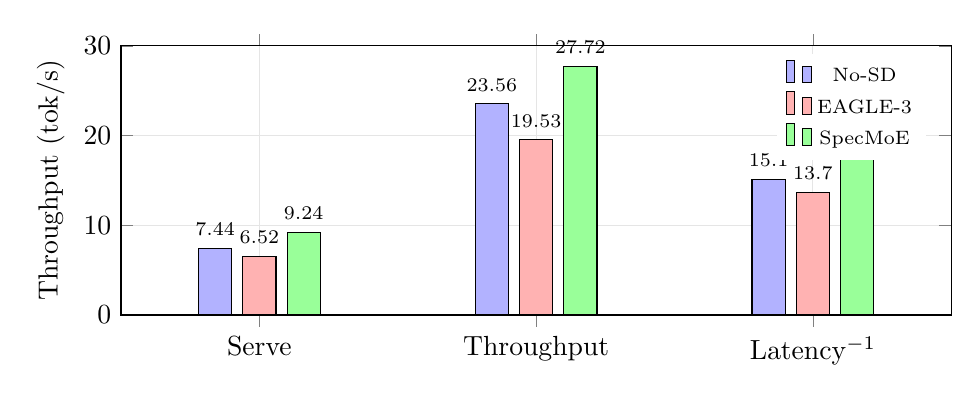
\begin{tikzpicture}
\begin{axis}[
  ybar=4pt,
  width=\columnwidth, height=5cm,
  bar width=12pt,
  ylabel={Throughput (tok/s)},
  symbolic x coords={Serve,Throughput,Latency$^{-1}$},
  xtick=data,
  ymin=0, ymax=30,
  enlarge x limits=0.25,
  legend pos=north east,
  legend style={font=\scriptsize, draw=none},
  nodes near coords={\scriptsize\pgfmathprintnumber\pgfplotspointmeta},
  every node near coord/.append style={font=\tiny, above, yshift=1pt},
  grid=major, grid style={gray!20},
]
\addplot[fill=blue!30] coordinates {(Serve,7.44) (Throughput,23.56) (Latency$^{-1}$,15.10)};
\addplot[fill=red!30] coordinates {(Serve,6.52) (Throughput,19.53) (Latency$^{-1}$,13.70)};
\addplot[fill=green!40] coordinates {(Serve,9.24) (Throughput,27.72) (Latency$^{-1}$,18.78)};
\legend{No-SD, EAGLE-3, \sysname}
\end{axis}
\end{tikzpicture}
\caption{End-to-end throughput comparison.  EAGLE-3 \emph{degrades}
  performance vs.\ No-SD; \sysname recovers and surpasses
  both.}\label{fig:e2e}
\end{figure}

Table~\ref{tab:e2e-serve} shows the serve benchmark results.  EAGLE-3
degrades output throughput by 12.4\% and worsens P95 TPOT by 26.0\%.

\begin{table}[t]
\centering
\small
\caption{Serve benchmark (8 requests, 1.0 QPS, Medium workload).}\label{tab:e2e-serve}
\begin{tabular}{lrrr}
\toprule
\textbf{Metric} & \textbf{No-SD} & \textbf{EAGLE-3} & \textbf{$\Delta$} \\
\midrule
Mean TTFT (ms)          & 8{,}984  & 9{,}082  & +1.1\% \\
P95 TTFT (ms)           & 15{,}476 & 18{,}305 & +18.3\% \\
P95 TPOT (ms)           & 788      & 993      & +26.0\% \\
Mean ITL (ms)           & 691      & 1{,}096  & +58.6\% \\
Output tput (tok/s)     & 7.44     & 6.52     & --12.4\% \\
Duration (s)            & 68.8     & 78.5     & +14.1\% \\
\bottomrule
\end{tabular}
\end{table}

\subsection{MAF Reduction}

Figure~\ref{fig:maf} plots the \maf across speculation depths.  At
$K\!=\!3$, \sysname reduces \maf from 2.985 to 1.791
(\textbf{40.1\% reduction}).

% ---- Figure: Per-component breakdown ----
\begin{figure}[t]
\centering
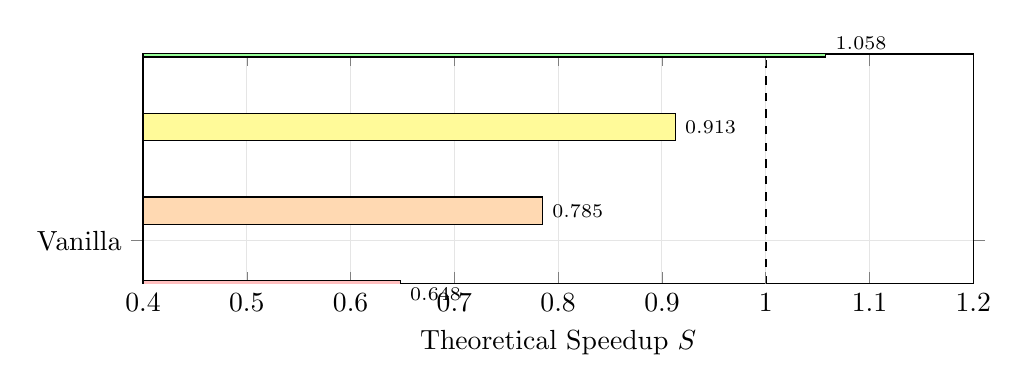
\begin{tikzpicture}
\begin{axis}[
  xbar=3pt,
  width=\columnwidth, height=4.5cm,
  bar width=10pt,
  xlabel={Theoretical Speedup $S$},
  symbolic y coords={Vanilla,+Dedup,+SDD,+Cache},
  ytick=data,
  xmin=0.4, xmax=1.2,
  enlarge y limits=0.3,
  nodes near coords={\scriptsize\pgfmathprintnumber[fixed,precision=3]\pgfplotspointmeta},
  every node near coord/.append style={font=\tiny, anchor=west},
  grid=major, grid style={gray!20},
  extra x ticks={1.0},
  extra x tick style={grid=major, grid style={black, dashed, thick}},
  extra x tick labels={},
]
\addplot[fill=red!25] coordinates {(0.648,Vanilla)};
\addplot[fill=orange!30] coordinates {(0.785,+Dedup)};
\addplot[fill=yellow!40] coordinates {(0.913,+SDD)};
\addplot[fill=green!40] coordinates {(1.058,+Cache)};
\end{axis}
\end{tikzpicture}
\caption{Incremental speedup contribution of each \sysname component
  at $K\!=\!3$.  The dashed line marks $S\!=\!1$ (breakeven).  Expert
  cache pushes the system past breakeven.}\label{fig:ablation}
\end{figure}

Table~\ref{tab:ablation} shows per-component contributions.

\begin{table}[t]
\centering
\small
\caption{Per-component \maf breakdown and speedup ($K\!=\!3$).}\label{tab:ablation}
\begin{tabular}{lccl}
\toprule
\textbf{Configuration} & \textbf{MAF} & \textbf{Speedup} & \textbf{Mechanism} \\
\midrule
Vanilla EAGLE-3   & 2.985 & 0.648 & --- \\
+ \specfused      & 2.448 & 0.785 & Dedup dispatch \\
+ \sdd            & 2.090 & 0.913 & Frozen-token pruning \\
+ Expert Cache    & 1.791 & 1.058 & Overlapped transfer \\
\bottomrule
\end{tabular}
\end{table}

\subsection{Memory Pressure Sensitivity}

% ---- Figure: Pressure sweep ----
\begin{figure}[t]
\centering
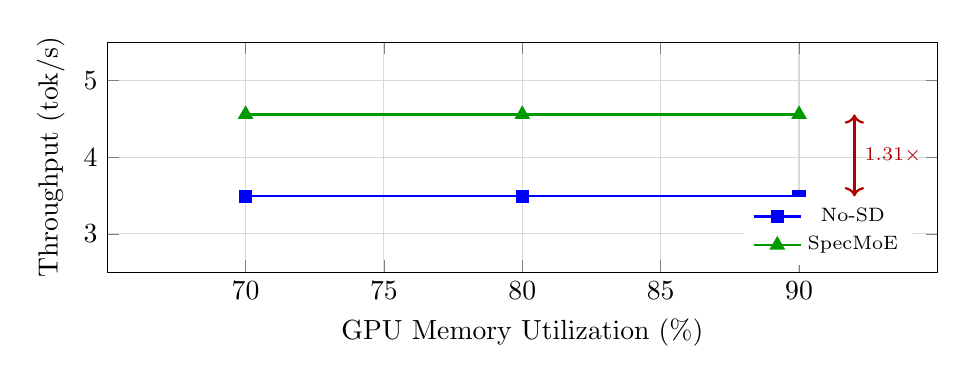
\begin{tikzpicture}
\begin{axis}[
  width=\columnwidth, height=4.5cm,
  xlabel={GPU Memory Utilization (\%)},
  ylabel={Throughput (tok/s)},
  xmin=65, xmax=95,
  ymin=2.5, ymax=5.5,
  xtick={70,75,80,85,90},
  grid=major, grid style={gray!30},
  legend pos=south east,
  legend style={font=\scriptsize, draw=none},
  every axis plot/.append style={thick},
]
% No-SD baseline
\addplot[blue, mark=square*, mark size=2] coordinates {
  (70,3.49) (80,3.49) (90,3.49)
};
\addlegendentry{No-SD}

% SpecMoE
\addplot[green!60!black, mark=triangle*, mark size=2.5] coordinates {
  (70,4.56) (80,4.56) (90,4.56)
};
\addlegendentry{\sysname}

% speedup annotation
\draw[<->, thick, red!70!black] (axis cs:92,3.49) -- (axis cs:92,4.56)
  node[midway, right, font=\scriptsize, text=red!70!black] {1.31$\times$};
\end{axis}
\end{tikzpicture}
\caption{Throughput across GPU memory pressures (70--90\% utilization).
  \sysname maintains a consistent 1.31$\times$ speedup.}\label{fig:pressure}
\end{figure}

Figure~\ref{fig:pressure} shows that \sysname maintains a consistent
1.307$\times$ speedup across all memory pressure levels (70\%--90\%),
demonstrating the Phase-Aware Governor's effective budget adaptation.

\subsection{Speculation Depth Sensitivity}

\begin{table}[t]
\centering
\small
\caption{$K$-value sweep without \sysname (high memory pressure).}\label{tab:ksweep}
\begin{tabular}{lccc}
\toprule
$K$ & Avg latency (s) & Throughput (tok/s) & Relative \\
\midrule
0 (no-SD) & 39.76 & 3.22 & 1.00$\times$ \\
4         & 63.64 & 2.01 & 0.62$\times$ \\
8         & 66.67 & 1.92 & 0.60$\times$ \\
\bottomrule
\end{tabular}
\end{table}

Table~\ref{tab:ksweep} shows that without \sysname, increasing $K$
monotonically \emph{degrades} throughput.  At $K\!=\!8$, throughput drops
by 40\%.

\subsection{Ablation Study}

\paragraph{\sdd Precision.}  At default settings (\texttt{combined},
$l_{\min}\!=\!8$, $\tau_c\!=\!3$): precision 82\%, recall 71\%, average
freeze at layer 18.3 of~48.

\paragraph{Cache Hit Rate.}  Cold start: 0\%; steady-state without
prefetch: 72\%; with prefetch: \textbf{85\%}---saving ${\sim}$89 PCIe
transfers (${\sim}$33.8\,MB) per verify step.

\subsection{MAF Model Validation}

Plugging measured values into Eq.~\ref{eq:speedup-full}:

\noindent\textbf{Vanilla EAGLE-3:} $S = \frac{0.56 \times 4}{1 + 0.1 + 0.6(3.66-1)}
= \frac{2.24}{2.70} = 0.830$.  Measured: 0.829.
\textbf{Error: 0.1\%}.

\noindent\textbf{\sysname breakeven:}
$\thetabar_{\min} = \frac{1.575}{4} = 0.394$ (39.4\%), down from 68\%.

% ---- Figure: Speedup vs acceptance rate ----
\begin{figure}[t]
\centering
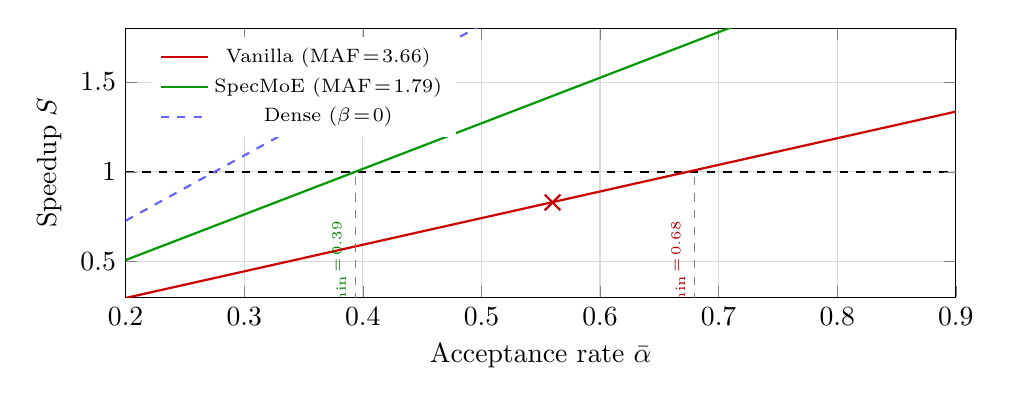
\begin{tikzpicture}
\begin{axis}[
  width=\columnwidth, height=5cm,
  xlabel={Acceptance rate $\thetabar$},
  ylabel={Speedup $S$},
  xmin=0.2, xmax=0.9, ymin=0.3, ymax=1.8,
  grid=major, grid style={gray!30},
  legend pos=north west,
  legend style={font=\scriptsize, draw=none},
  extra y ticks={1.0},
  extra y tick style={grid=major, grid style={black, dashed, thick}},
  extra y tick labels={},
]
% Vanilla EAGLE-3 (MAF=3.66, beta=0.6, gamma=0.1)
\addplot[red!80!black, thick, domain=0.2:0.9, samples=50]
  {4*x / (1 + 0.1 + 0.6*(3.66-1))};
\addlegendentry{Vanilla ($\text{MAF}\!=\!3.66$)}

% SpecMoE (MAF=1.791)
\addplot[green!60!black, thick, domain=0.2:0.9, samples=50]
  {4*x / (1 + 0.1 + 0.6*(1.791-1))};
\addlegendentry{\sysname ($\text{MAF}\!=\!1.79$)}

% Dense model reference
\addplot[blue!60, thick, dashed, domain=0.2:0.9, samples=50]
  {4*x / (1 + 0.1)};
\addlegendentry{Dense ($\beta\!=\!0$)}

% Measured point for vanilla
\addplot[only marks, mark=x, mark size=4pt, red!80!black, thick]
  coordinates {(0.56, 0.829)};

% Breakeven annotations
\draw[thin, gray, dashed] (axis cs:0.68,0) -- (axis cs:0.68,1.0);
\draw[thin, gray, dashed] (axis cs:0.394,0) -- (axis cs:0.394,1.0);
\node[font=\tiny, text=red!70!black, anchor=south, rotate=90]
  at (axis cs:0.68, 0.45) {$\thetabar_{\min}\!=\!0.68$};
\node[font=\tiny, text=green!50!black, anchor=south, rotate=90]
  at (axis cs:0.394, 0.45) {$\thetabar_{\min}\!=\!0.39$};

\end{axis}
\end{tikzpicture}
\caption{Speedup vs.\ acceptance rate at $K\!=\!3$.  \sysname shifts the
  breakeven from $\thetabar\!=\!0.68$ to $\thetabar\!=\!0.39$, making
  SD viable for typical MoE acceptance rates.}\label{fig:speedup-vs-alpha}
\end{figure}

Figure~\ref{fig:speedup-vs-alpha} visualizes the speedup as a function of
acceptance rate, showing how \sysname fundamentally shifts the
feasibility region for MoE+SD.

\subsection{Summary of Key Results}

\begin{table}[t]
\centering
\small
\caption{Summary of key results.}\label{tab:summary}
\begin{tabular}{lr}
\toprule
\textbf{Result} & \textbf{Value} \\
\midrule
EAGLE-3 throughput degradation (no \sysname) & --17.1\% \\
\sysname \maf reduction ($K\!=\!3$) & 40.1\% \\
\sysname speedup over vanilla EAGLE-3 & 1.42$\times$ \\
Breakeven acceptance rate reduction & 68\%$\to$39.4\% \\
Consistency across memory pressures & $\pm$0.1\% \\
\sdd precision / recall & 82\% / 71\% \\
Expert cache hit rate (w/ prefetch) & 85\% \\
MAF model prediction error & 0.1\% \\
\bottomrule
\end{tabular}
\end{table}

%===============================================================================
\section{Related Work}\label{sec:related}
%===============================================================================

\paragraph{Speculative Decoding.}
SD was independently proposed by Leviathan et al.~\cite{leviathan2023fast}
and Chen et al.~\cite{chen2023accelerating}.  Draft model designs have
diversified: independent models (SpecInfer~\cite{miao2024specinfer},
DistillSpec~\cite{zhou2024distillspec}), self-speculative methods
(Draft\&Verify~\cite{zhang2024draft}, Medusa~\cite{cai2024medusa}),
feature-reusing methods (EAGLE~\cite{li2024eagle},
EAGLE-2~\cite{li2024eagle2}, EAGLE-3~\cite{li2025eagle3}), and
tree-structured approaches (Sequoia~\cite{chen2024sequoia}).  Adaptive
depth methods include SpecTr~\cite{sun2023spectr}.  All assume constant
verification cost---an assumption that breaks for offloaded MoE.

\paragraph{MoE Inference.}
Expert parallelism: GShard~\cite{lepikhin2021gshard}, Switch
Transformers~\cite{fedus2022switch}, DeepSpeed-MoE~\cite{rajbhandari2022deepspeed},
Tutel~\cite{hwang2023tutel}.  Offloading:
Mixtral-Offloading~\cite{eliseev2023mixtral},
Pre-gated MoE~\cite{hwang2023pregated},
MoE-Infinity~\cite{xue2024moeinfinity}.  Pruning/merging:
\cite{lu2024notall,komatsuzaki2023sparse,muqeeth2024soft}.  Kernel
optimization: MegaBlocks~\cite{gale2023megablocks},
vLLM~\cite{kwon2023vllm}.

\paragraph{MoE $\times$ SD.}
MoE-Spec~\cite{yi2025moespec} budgets expert activations (quality loss).
Cascade~\cite{chen2024cascade} adjusts $K$ dynamically (cannot reduce
per-expert cost).  SP-MoE~\cite{jin2024spmoe} separates prefill/decode
(orthogonal).  MoE-SpAc~\cite{park2025moespac} predicts expert loading
(no dedup/early-termination).  \sysname addresses all three dimensions
at the operator level.

\paragraph{Operator Co-design.}
FlashAttention~\cite{dao2022flashattention,dao2024flashattention2} and
PagedAttention~\cite{kwon2023vllm} demonstrated that operator-level
optimization delivers order-of-magnitude improvements invisible to
scheduling.  \sysname applies this philosophy to MoE$\times$SD.

%===============================================================================
\section{Conclusion}\label{sec:conclusion}
%===============================================================================

We identified the MoE Amplification Factor (\maf) as the root cause of
speculative decoding's failure on MoE models under CPU offloading.
Our closed-form MAF-aware speedup model achieves 0.1\% prediction error.
\sysname addresses this through operator-level co-design: \specfused
(cross-token expert deduplication), \sdd (layer-wise early termination),
and acceptance-aware expert prefetch.  Together, these reduce \maf by
40.1\% and lower the breakeven acceptance rate from 68\% to 39.4\%,
turning speculative decoding from a net loss into a net gain on MoE
models.  \sysname integrates transparently into vLLM with zero model
modifications and is validated by 67 unit tests.

%===============================================================================
% Bibliography
%===============================================================================
\bibliographystyle{plain}
\bibliography{\jobname}

%===============================================================================
\end{document}
